\section{Performance Assessment}
\label{2017-coo-spmv:s4-experiments}

\begin{figure}
\begin{center}
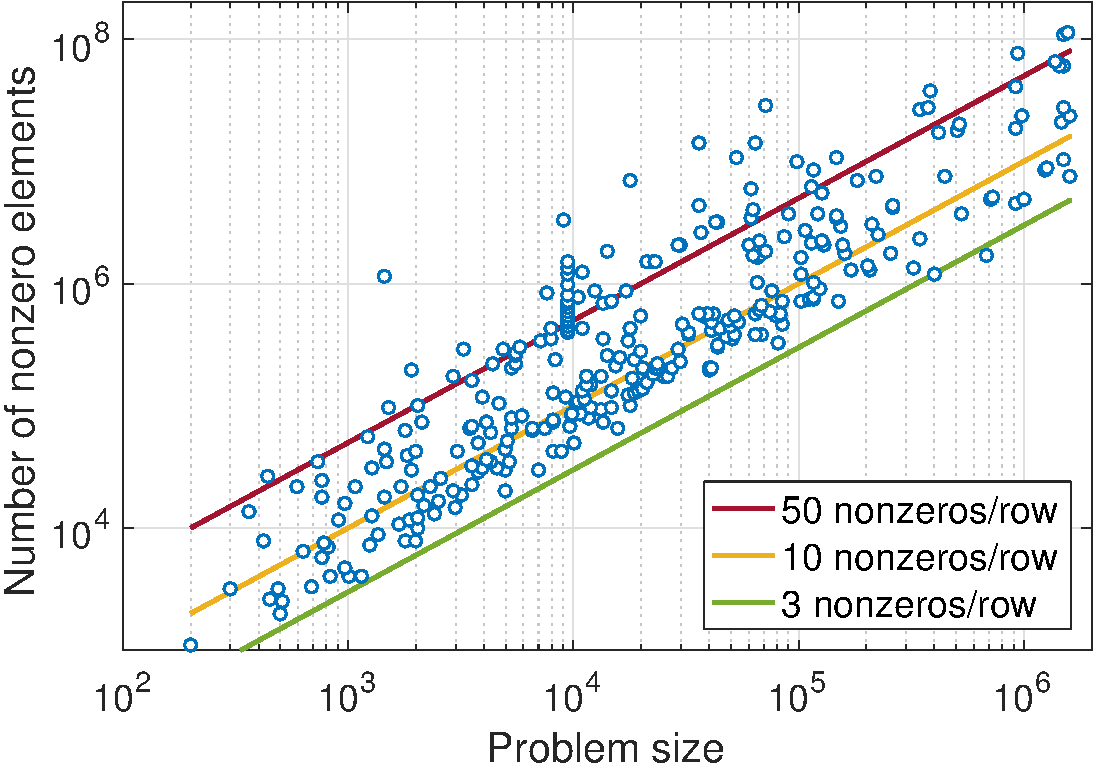
\includegraphics[width=\columnwidth]{plots/matrixchar_nnz}
\end{center}
\caption{Nonzero count vs. size for the considered test matrices. 
For convenience we added density baselines for 3 nnz/row, 10 nnz/row, and 50 nnz/row.
}
\label{2017-coo-spmv:fig:matrixnnz}
\end{figure}


\begin{figure}
\begin{center}
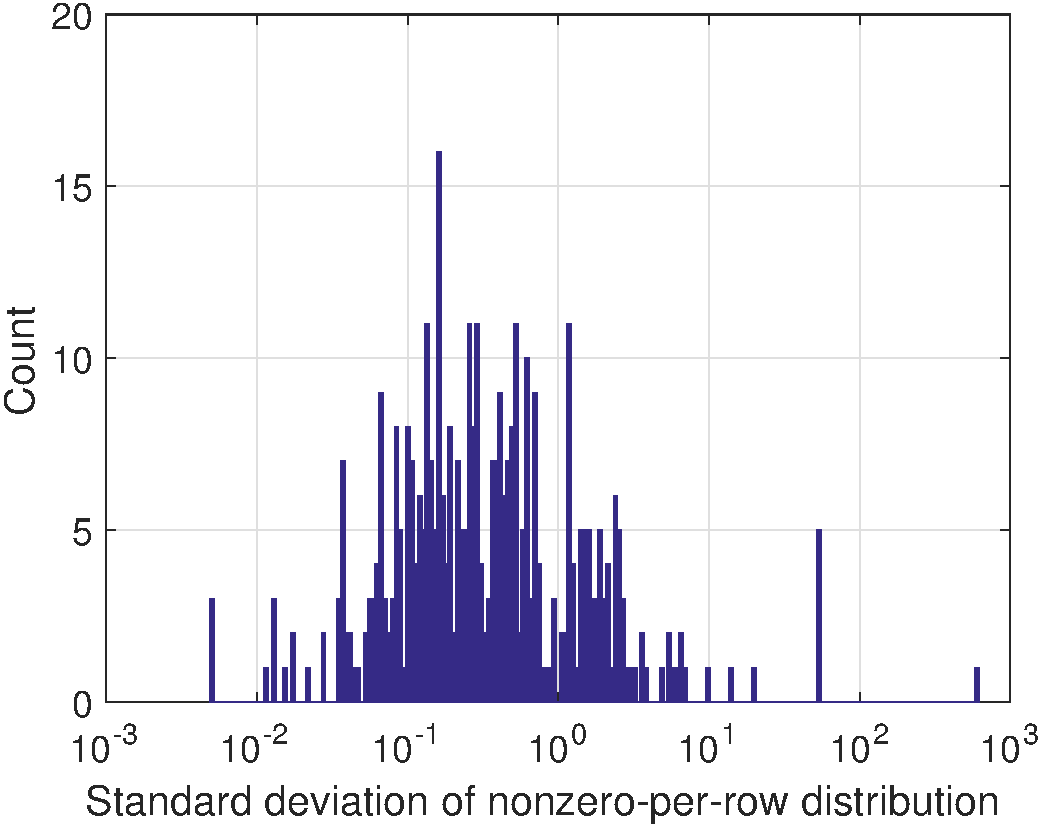
\includegraphics[width=\columnwidth]{plots/matrixchar_std_avg_logy}
\end{center}
\caption{Histogram for the ( standard deviation / avg ) of the nonzero-per-row metric. Few problems have a higher standard deviation than $10^2$.}
\label{2017-coo-spmv:fig:matrixstd}
\end{figure}

\begin{figure*}
\begin{center}
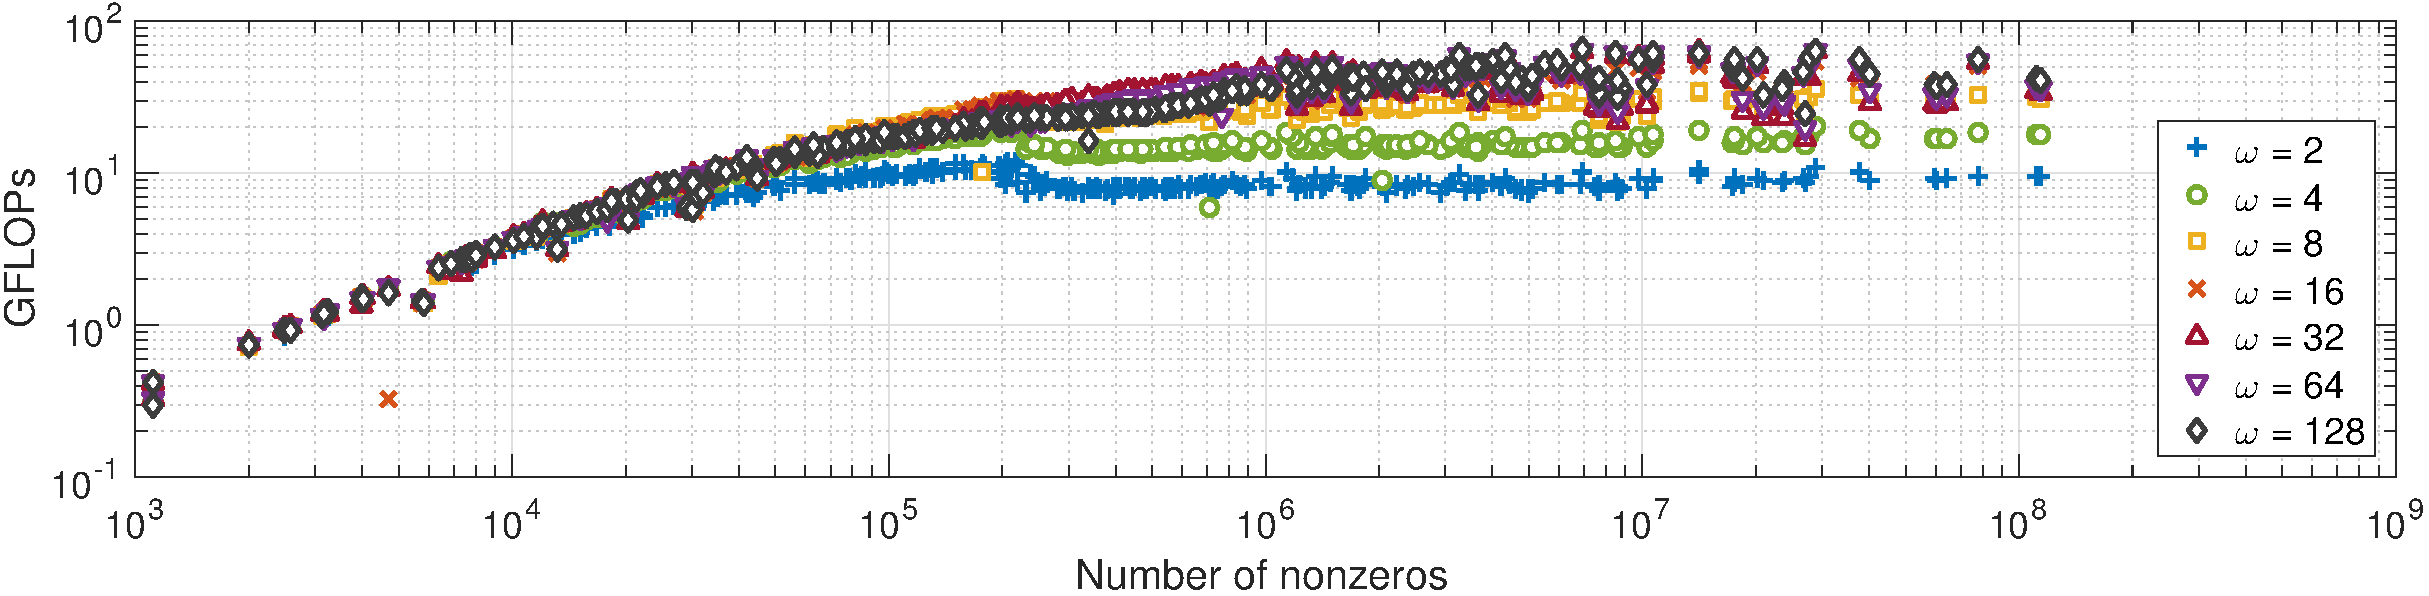
\includegraphics[width=\columnwidth]{plots/COO_GFLOPS_nnz}
\end{center}
\caption{Evaluating the effect of the parameter $\omega$ on the performance of the \coo kernel. The matrices are ordered according to increasing nonzero count.}
\label{2017-coo-spmv:fig:COOanalysis}
\end{figure*}

\begin{figure*}
\begin{center}
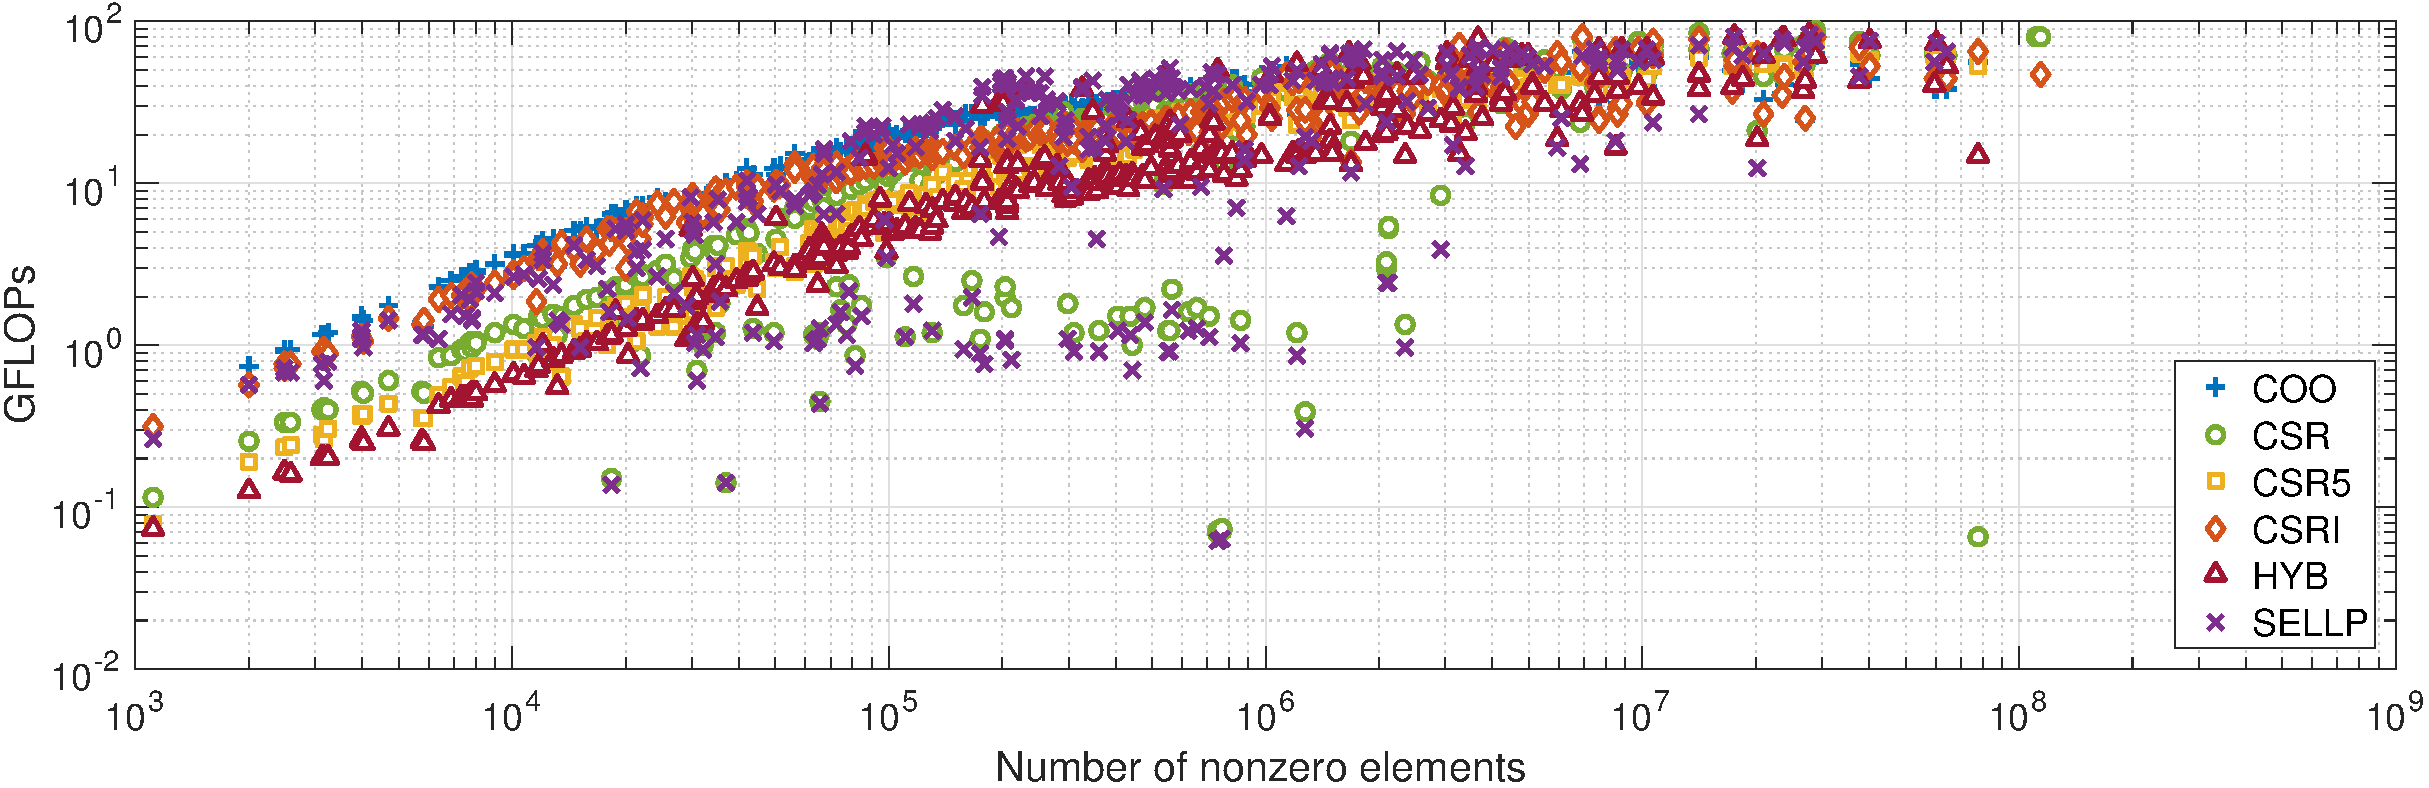
\includegraphics[width=\columnwidth]{plots/GFLOPS_all_nnz_nnz}
\end{center}
\caption{Performance of the distinct \spmv kernels for all problems included in the test suite. The matrices are ordered according to increasing nonzero count.}
\label{2017-coo-spmv:fig:GFLOPsnnz}
\end{figure*}


\subsection{Test matrices}
For the experimental performance analysis, we use a set of 400 matrices from the
SuiteSparse matrix collection~\cite{ufmc}. This collection 
comprises a large number of matrices that differ in the algebraic field (real, complex, pattern),
the shape (square, rectangular), and matrix-specific characteristics such as
size and nonzero pattern.
For the performance assessment we focus on real, square matrices that have a pairwise different nonzero pattern.
In Figure~\ref{2017-coo-spmv:fig:matrixnnz} we visualize the size and nonzero count of the chosen test matrices. 
In order to quantify the imbalance of the nonzero distribution of a matrix,
we use the standard deviation of the nonzero-per-row metric, see Figure~\ref{2017-coo-spmv:fig:matrixstd}.

\subsection{Experiment setup}
All experiments were conducted on the GPU-accelerated compute nodes of the 
PizDaint supercomputer at the Swiss National Computing Centre (CSCS). 
Although irrelevant for the performance analysis, we mention that the host composes of
an Intel E5-2690 v3 processor (codename Haswell) with 12 cores running at 2.6 GHz.
All computations are executed by the NVIDIA Tesla P100 GPU (compute capability 6.0)
for which NVIDIA lists a double precision peak performance of 5.3 TFLOPs ($10^{12}$ floating point operations per second). 
We use double precision in all experiments.
The P100 is equipped with 16 GB main memory, which
is accessed at a theoretical bandwidth of 732 GB/s.
Using the bandwidth test that ships with CUDA 8.0 (and that puts equal pressure 
on memory reads and memory writes) we were able to achieve 497 GB/s.
Using NVIDIA's CUDA toolkit version 8.0, we design the \coo kernel to
integrate into the MAGMA-sparse software library~\cite{parco2017}.
MAGMA-sparse is also used as experiment ecosystem, and provided
the  \spmv reference implementations. Specifically, the reference implementations are:
\begin{enumerate}
\item[\csr]
The CSR-based \spmv kernel we consider is part of NVIDIA's cuSPARSE library.
\item[\csrfive]
The \csrfive \spmv kernel is based on modifying the CSR format for achieving higher performance. The implementation is part of the MAGMA-sparse software stack, 
details about the kernel are presented in Liu et 
al.~\cite{Liu:2015:CES:2751205.2751209}.
\item[\csri]
The design of the \csri \spmv kernel is very similar to the \coo kernel we propose. 
It tries to enable load balancing for unbalanced matrices stored in CSR by
using atomic addition operations~\cite{csri}.  
\item[\hyb]
The hybrid \spmv kernel we consider combines the ELL format for the regular (balanced) part
of the matrix with the COO format for the irregular part of the matrix. We use the implementation available in NVIDIA's cuSPARSE library.
\item[\sellp]
The SELL-p kernel is also part of the MAGMA-sparse software ecosystem,
and has proven to be very efficient for balanced problems~\cite{sellc}.
\end{enumerate}

\subsection{Experimental results}
In a first experiment, we analyze the effect of the oversubscribing-parameter $\omega$ 
on the performance of the \coo kernel.
In Figure~\ref{2017-coo-spmv:fig:COOanalysis} we order the matrices for increasing nonzero count, 
and report the performance for the $\omega$-values 2, 4, 8, 16, 32, 64, and 128.
We notice that the performance differences increase with the
nonzero count. For small nonzero counts, the differences are negligible. 
The optimal choice for the $\omega$ parameter then takes turns: 
Moderate oversubscribing with $\omega=8$/$\omega=16$ 
is the performance winner for systems with about $10^5$ nonzeros,
$\omega=32$/$\omega=64$ is superior for systems with about $10^6$ nonzeros,
and $\omega=128$ seems to be the best parameter choice beyond that.
The nonzero count of a matrix is one of the characteristics known prior
to the \spmv invocation. 
Hence, a straight-forward optimization step for the \coo kernel is given 
by choosing $\omega$ on a heuristic derived from Figure~\ref{2017-coo-spmv:fig:COOanalysis}.
In the rest of the paper we define the \coo as the kernel that chooses 
\[
\omega =
\begin{cases}
\begin{array}{lll}
8 & \mathrm{\ for\ } & nnz<10^5,\\
32 & \mathrm{\ for\ } & 10^5 \leq nnz<10^6,\\
128 & \mathrm{\ for\ }&10^6 \leq nnz.
\end{array}
\end{cases}
\]

Next, we compare the \coo kernel with the reference kernels previously listed. 
In Figure~\ref{2017-coo-spmv:fig:GFLOPsnnz} we order the test matrices according to increasing nonzero count,
and visualize the performance of all \spmv kernels we consider in this analysis. 

Independent of the \spmv kernel, the performance linearly increases with the nonzero count of the problems until it stagnates around 90 GFLOPs. 

Furthermore, the visualization suggests that the \coo kernel is the fastest kernel for almost 
all test matrices
with less than $2 \cdot 10^5$ nonzero elements. For problems containing more nonzero elements it
is difficult to identify an overall winner. This is partly because multiple
performance indicators are covering each other, and distinct problems, although different in
sparsity pattern, may have the same nonzero count, and are therefore arranged in the same place on the x-axis. 
Overall, it is difficult to extract from this figure for how many problems a specific kernel is the fastest. 
We answer this question in Figure~\ref{2017-coo-spmv:fig:stats} where we report for how many problems a certain kernel was the performance winner (blue bar) and for how many problems a certain kernel gave the worst performance (red bar). If the kernel was neither the fastest nor the slowest for a certain problem, it is counted as ``ballpark.'' In the end, for each kernel we get a bar of the same length split into three colors; the sum of all blue parts and the sum of all red parts equals the number of test cases, respectively.

\begin{figure}
\begin{center}
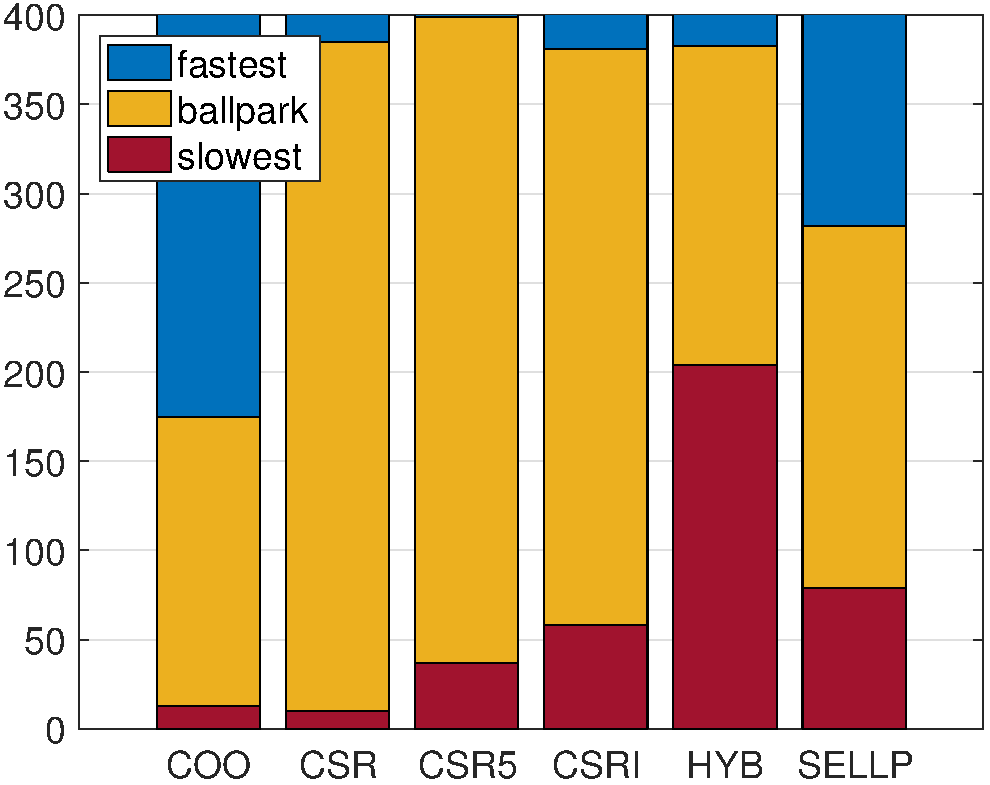
\includegraphics[width=\columnwidth]{plots/stats0}
%\includegraphics[width=.8\columnwidth]{plots/stats_2e5}
\end{center}
\caption{Fastest kernel comparison: blue bars represent the number of problems
    for which the kernel was the fastest, red bars count the problems for which
    the kernel was the slowest in the comparison.}
\label{2017-coo-spmv:fig:stats}
\end{figure}

\begin{figure}
\begin{center}
%\includegraphics[width=.8\columnwidth]{plots/boxplot_log_csri}
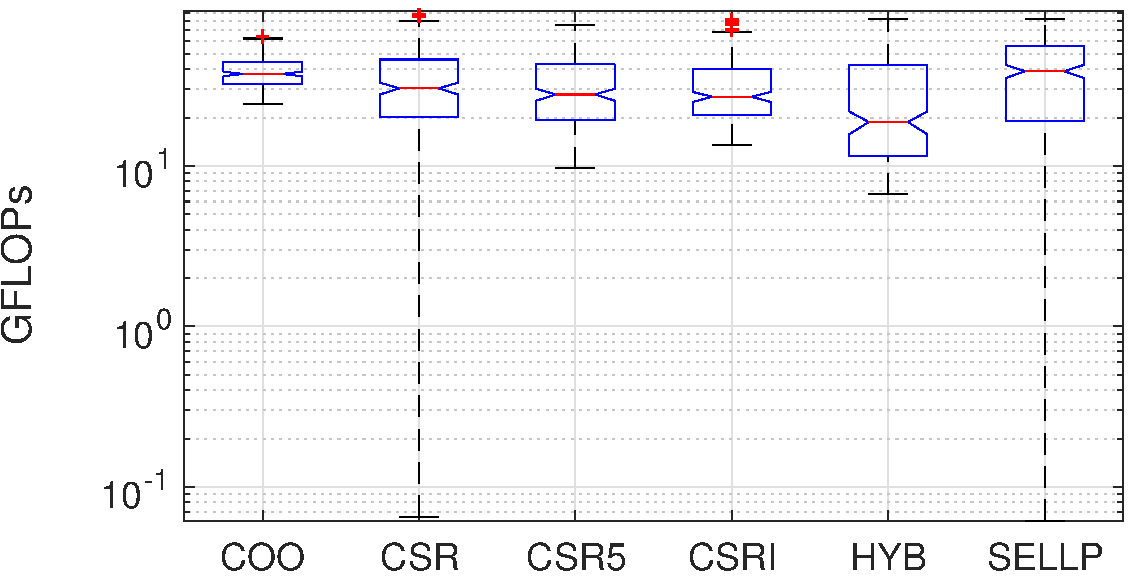
\includegraphics[width=\columnwidth]{plots/boxplot_log_csri_2e5}
\end{center}
\caption{Performance statistics for the distinct kernels over the test cases containing more than $2\cdot 10^5$ nonzero elements.}
\label{2017-coo-spmv:fig:boxplot}
\end{figure}

\begin{table}
\begin{center}
\begin{tabular}{lrrrrrr}
\hline
\hline
Kernel & min & max & average & median & standard-dev.\\
\hline
\coo &    24.29 &    64.32 &    38.86 &    37.24 &     9.16 & \\
\csr &     0.07 &    87.43 &    32.77 &    30.43 &    20.07 & \\
\csrfive &     9.66 &    75.56 &    31.79 &    27.15 &    15.58 & \\
\csri &    13.47 &    81.21 &    31.85 &    26.84 &    14.44 & \\
\hyb &     6.64 &    82.43 &    27.98 &    18.74 &    20.22 & \\
\sellp &     0.06 &    82.62 &    36.42 &    38.64 &    22.46 & \\
\hline
\hline
\end{tabular}
\end{center}
\caption{Statistical information on the GFLOPs metric of the \spmv kernel
for the 248 matrices containing more than $2\cdot 10^5$ nonzero elements.}
\label{2017-coo-spmv:tab:stats}
\end{table}

\begin{figure*}
\begin{center}
%\includegraphics[width=2.0\columnwidth]{plots/overhead_log}
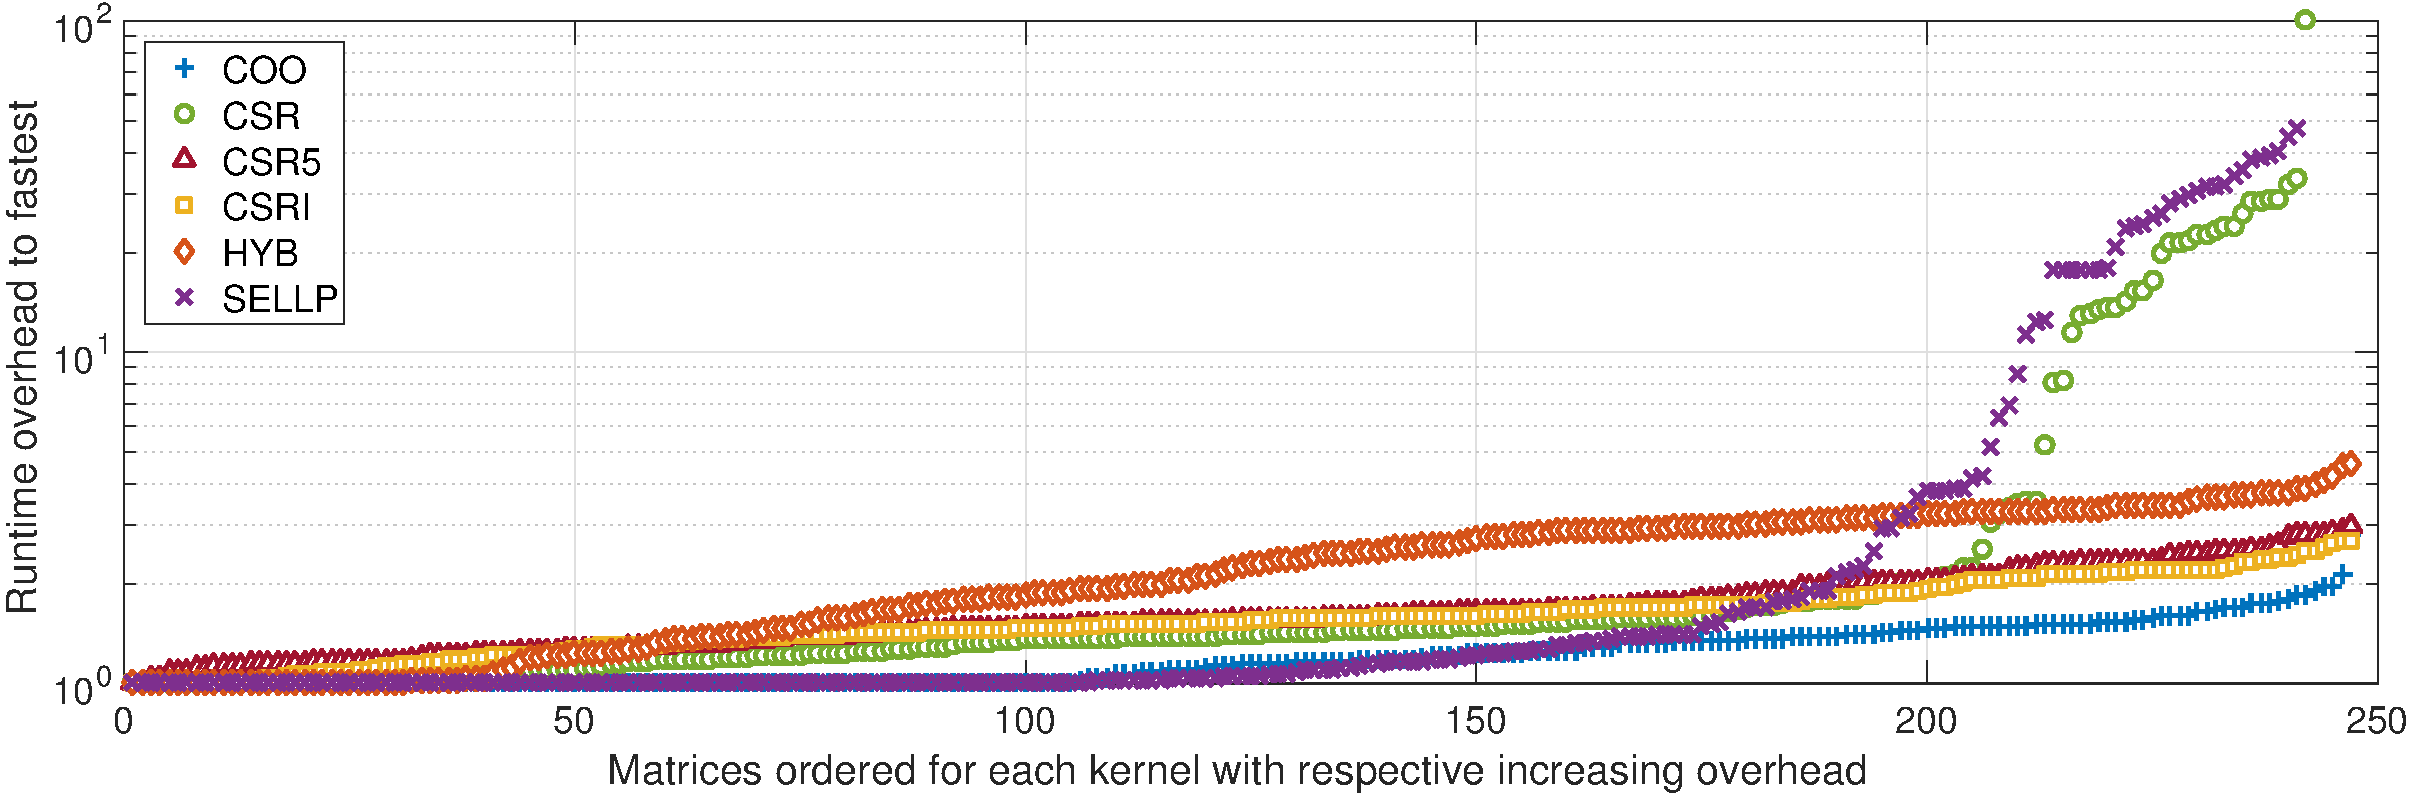
\includegraphics[width=\columnwidth]{plots/overhead_log_2e5}
\end{center}
\caption{Runtime overhead of the distinct \spmv kernels. For each kernel, the matrices are ordered with respect to increasing overhead. Only test matrices with more than $2\cdot 10^5$ nonzero elements are considered.}
\label{2017-coo-spmv:fig:overhead}
\end{figure*}

Overall, the \coo kernel wins most cases, and it is followed by the \sellp
\spmv. \csr, \csri, and \hyb win only few cases, \csrfive not a single one. On
the other hand, \csrfive and \csr are rarely the slowest kernels, while
\coo, \csri, \sellp, and \hyb lose significantly more cases.

Looking at the complete test suite containing all 400 matrices, 
we include problems that are ``small'' with respect to the computational workload of the \spmv.
For those, even the winning kernel in Figure~\ref{2017-coo-spmv:fig:stats} achieves 
only low execution performance. 
In scientific applications, these ``easy'' problems are typically rather handled via a direct solver
than an iteration method based on the \spmv kernel.
As we are in particular interested in the performance for problems 
that are the characteristic target we limit the further analysis to the 248 
problems containing more than $2\cdot 10^5$ nonzero elements.

In Figure~\ref{2017-coo-spmv:fig:boxplot} we compare the distinct \spmv kernels in the GFLOPs 
metric for the problems containing more than $2\cdot 10^5$ nonzero elements.
We accompany this graph with some numeric information in 
Table~\ref{2017-coo-spmv:tab:stats} where we additionally 
list the average performance. 
For this metric, the \coo format turns out to be the
overall winner with an average 38.86 GFLOPs.
Looking at the median, the \sellp and \coo kernels 
achieve the highest execution rate (38.64 GFLOPs and 37.24 GFLOPs, respectively).
They outperform the closest competitor \csr by about 25\%.
The lowest median performance of 18.74 GFLOPs is achieved by the \hyb kernel.
At the same time, the \hyb kernel achieves significantly higher performance 
(up to 82.43 GFLOPs) for specific test cases, see Table~\ref{2017-coo-spmv:tab:stats}.
Only the \sellp and the \csr kernel achieve higher performance for balanced and regular 
problems (82.62 GFLOPs and 87.43 GFLOPs, respectively).

Most noticeable in Figure~\ref{2017-coo-spmv:fig:boxplot} 
is the variation of the \coo performance being radically smaller than
for any of the other formats: 
50\% of the performance numbers are within a 6 GFLOP/s range from the median,
the standard deviation is 9.16. 
The lowest performance number for the \coo kernel is 24 GFLOPs.
Only the \csri kernel is competitive in handling unbalanced problems,
with 50\% of the performance numbers between 20 GFLOPs and 60 GFLOPs,
a standard deviation of 14.44, and the lowest performance being 13.47 GFLOPs 
(see Table~\ref{2017-coo-spmv:tab:stats}).
For \sellp and \csr, the performance values spread across a large range.
In particular, 
the lowest performance numbers (0.06 GFLOPs for \sellp and 0.07 GFLOPs for \csr) 
are far from the median. 
The central box (upper/lower quantiles)
are for these kernels a multiple of those for \coo. 
Also the upper and lower whiskers are significantly further apart.
For \sellp, this is expected as, for unbalanced matrices, the nonzero padding to a
block-uniform nonzero count introduces significant performance-detrimental
overhead, as well as load imbalance in-between the matrix blocks.
Load imbalance is also the culprit for \csr's poor performance.
Hence, the formats delivering the best performance for balanced test matrices
are not suitable for irregular unbalances problems.
The \coo format, although achieving only 64.32 GFLOPs for the best case,
proves to handle irregular problems well, with the highest average performance,
a competitive median, the smallest
variation, and the highest minimal performance.

Finally, we want to assess the performance penalty of choosing one specific kernel
vs. choosing the problem-specific best kernel.
Obviously, the problem-specific best format is unknown a priori, and one would have 
to test all kernels prior to the the performance-relevant run, or use machine learning techniques
for making a good guess. 
Again, we focus on the problems containing more than $2\cdot 10^5$ nonzero elements.
In the analysis we identify the optimal format for each test matrix,
and scale the performance of all kernels to this baseline.
We then sort the matrices with increasing overhead for every kernel
individually, and visualize this characteristic curve in
Figure~\ref{2017-coo-spmv:fig:overhead}. 
Hence, the order of the matrices is different for each kernel,
but the overheads are increasing in all datasets.
The objective of minimizing the slowdown corresponds to minimizing the area
below the curve. The longer a curve stays at 1, the more test cases a certain
kernel wins.
We notice that the overhead stays low particularly for \coo, \csri, and \csrfive.
For \sellp and \csr, the initially moderate overhead for balanced problems 
quickly grows for irregular problems.
\hyb deals better with these cases, however it already starts of with a larger overhead than 
\coo and the CSR variants.
Overall, \coo has a radically lower overhead than any of the competitors.
Another key observation is that (ignoring two outliers) the \coo kernel never
exhibits a slowdown factor larger than two. This implies that choosing the \coo
format results in an \spmv kernel which is in the worst case two times slower
than the (unknown) optimal choice. 
This clearly makes \coo the overall winner in this metric as well.
